%%%%%%%%%%%%%%%%%%%%%%%%%%%%%%%%%%%%%%%%%
% Poster for the PaPE Conference 2017 by Bradley Rentz and Victoria Anderson
% Code adapted from:
% baposter Landscape Poster
% LaTeX Template
% Version 1.0 (11/06/13)
%
% baposter Class Created by:
% Brian Amberg (baposter@brian-amberg.de)
%
% This template has been downloaded from:
% http://www.LaTeXTemplates.com
%
% License:
% CC BY-NC-SA 3.0 (http://creativecommons.org/licenses/by-nc-sa/3.0/)
%
%%%%%%%%%%%%%%%%%%%%%%%%%%%%%%%%%%%%%%%%%

%----------------------------------------------------------------------------------------
%	PACKAGES AND OTHER DOCUMENT CONFIGURATIONS
%----------------------------------------------------------------------------------------

% Note: to compile need fonts: Source Sans Pro & Univers LT Std

\documentclass[portrait,fontscale=0.285,a0paper]{baposter2}
 % Adjust the font scale/size here
 
\usepackage{wrapfig}

\usepackage{graphicx} % Required for including images
\graphicspath{{figures/}} % Directory in which figures are stored

\usepackage{amsmath} % For typesetting math
\usepackage{amssymb} % Adds new symbols to be used in math mode

\usepackage{booktabs} % Top and bottom rules for tables
\usepackage{enumitem} % Used to reduce itemize/enumerate spacing
%\usepackage{palatino} % Use the Palatino font
\usepackage[font=small,labelfont=bf]{caption} % Required for specifying captions to tables and figures

\usepackage{multicol} % Required for multiple columns
\setlength{\columnsep}{1.5em} % Slightly increase the space between columns
\setlength{\columnseprule}{0mm} % No horizontal rule between columns

\usepackage{subcaption}
\usepackage{setspace}

\usepackage{tikz} % Required for flow chart
\usetikzlibrary{shapes,arrows} % Tikz libraries required for the flow chart in the template

\newcommand{\compresslist}{ % Define a command to reduce spacing within itemize/enumerate environments, this is used right after \begin{itemize} or \begin{enumerate}
\setlength{\itemsep}{1pt}
\setlength{\parskip}{0pt}
\setlength{\parsep}{0pt}
}
\usepackage{natbib}
\bibpunct[: ]{(}{)}{,}{a}{}{,}
	\newcommand{\BIBand}{\&}
	\setlength{\bibsep}{0pt}
	\setlength{\bibhang}{0.25in}
	\bibliographystyle{sp}



\usepackage{fontspec}
\newcommand{\timesm}{\fontspec[
Contextuals={Inner,WordFinal,WordInitial},Ligatures={Common,TeX}]{Roboto Light}\fontsize{10pt}{13.5pt}\selectfont}%

\newcommand{\sansipa}{\fontspec[
Contextuals={Inner,WordFinal,WordInitial},Ligatures={Common,TeX}]{Roboto Light}\fontsize{15pt}{13.5pt}\selectfont}%

\usepackage[activate={true},
  final,
  tracking=true, % breaks sc
  factor=1200,
  stretch=50,
  shrink=0
  ]{microtype}

\pdfprotrudechars=2
\pdfadjustspacing=2
\newfontfeature{Microtype}{protrusion=default;expansion=default}
\directlua{fonts.protrusions.setups.default.factor=.5}
\defaultfontfeatures{Mapping=text-text}

\setmainfont[BoldFont={Roboto Medium},Contextuals={Inner,WordFinal,WordInitial},ItalicFont={Roboto Light Italic},Ligatures={Common,TeX}]{Roboto Light}\fontsize{9.5pt}{13pt}

\newcommand{\ipa}{\fontspec[
Contextuals={Inner,WordFinal,WordInitial},Ligatures={Common,TeX}]{Roboto Light}\fontsize{9.5pt}{13pt}\selectfont}

\newcommand{\mainfont}{\fontspec[BoldFont={Roboto Medium},
Contextuals={Inner,WordFinal,WordInitial},Ligatures={Common,TeX},ItalicFont={Roboto Light Italic}]{Roboto Light}\fontsize{9.5pt}{13pt}\selectfont}

\newcommand{\georgianfont}{\fontspec[BoldFont={Roboto Medium},
Contextuals={Inner,WordFinal,WordInitial},Ligatures={Common,TeX},ItalicFont={Roboto Light Italic}]{Helvetica Neue}\fontsize{8pt}{13pt}\selectfont}


\definecolor{lightblue}{RGB}{2,71,49} % Defines the color used for content box headers

\begin{document}
\mainfont
\begin{poster}
{
headerborder=closed, % Adds a border around the header of content boxes
colspacing=1em, % Column spacing
bgColorOne=white, % Background color for the gradient on the left side of the poster
bgColorTwo=white, % Background color for the gradient on the right side of the poster
borderColor=lightblue, % Border color
headerColorOne=darkgray, % Background color for the header in the content boxes (left side)
headerColorTwo=lightblue, % Background color for the header in the content boxes (right side)
headerFontColor=white, % Text color for the header text in the content boxes
boxColorOne=white, % Background color of the content boxes
textborder=roundedleft, % Format of the border around content boxes, can be: none, bars, coils, triangles, rectangle, rounded, roundedsmall, roundedright or faded
eyecatcher=true, % Set to false for ignoring the left logo in the title and move the title left
headerheight=0.1\textheight, % Height of the header
headershape=roundedright, % Specify the rounded corner in the content box headers, can be: rectangle, small-rounded, roundedright, roundedleft or rounded
headerfont=\mainfont\Large\bf, % Large, bold and sans serif font in the headers of content boxes
%textfont={\setlength{\parindent}{1.5em}}, % Uncomment for paragraph indentation
linewidth=2pt % Width of the border lines around content boxes
}
%----------------------------------------------------------------------------------------
%	TITLE SECTION 
%----------------------------------------------------------------------------------------
%
{
\includegraphics[height=8em]{seal.jpg}} % First university/lab logo on the left
{\bf\huge Tsova-Tush Language Attitudes and Use\\ \vspace{0.2em}}% Poster title
{Bryn Hauk \& Bradley Rentz \\ \vspace{0.1em} \emph{University of Hawai`i at M{\=a}noa, Department of Linguistics}} % Author names and institution
%{\includegraphics[height=4em]{logo.png}} % Second university/lab logo on the right

%----------------------------------------------------------------------------------------
%	OBJECTIVES
%----------------------------------------------------------------------------------------

\headerbox{Introduction}{name=objectives,column=0,row=0,span=1}{

\begin{singlespace}This poster provides updated information about the vitality of Tsova-Tush (Batsbi) [bbl], a Northeast
Caucasian language spoken  in the village of Zemo Alvani, Georgia. We re-estimate speaker numbers and report findings from a language use and attitude survey.\end{singlespace} %Given the language's status as severely endangered, the lack of 
%accurate information on its vitality is alarming. 



\vspace{0.3em} % When there are two boxes, some whitespace may need to be added if the one on the right has more content
}

%%%%%%


\headerbox{Map}{name=results,column=0,below=objectives,span=1}{
%Today Tsova-Tush is spoken exclusively in the village of Zemo Alvani, Georgia.\\
\begin{center}

  \vspace{-0.35in} 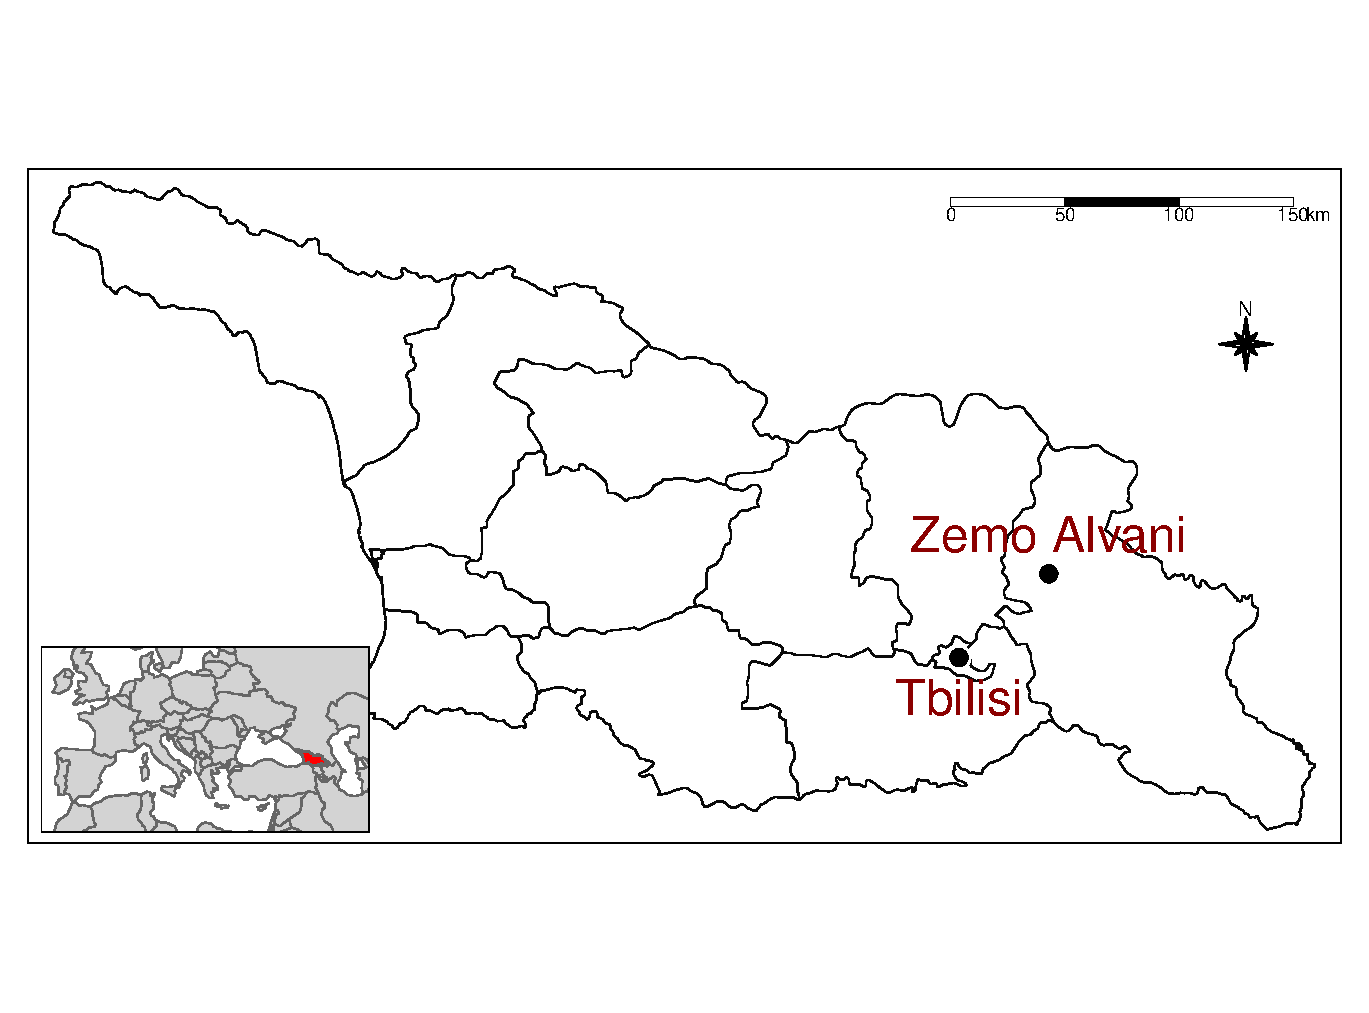
\includegraphics[width=1\textwidth]{georgia.pdf} \vspace{-0.65in}\captionof{figure}{\footnotesize Location of Zemo Alvani, Georgia where Tsova-Tush is spoken}
\end{center}

%\vspace{0.1in}{\large Estimated Tsova-Tush heritage population:}\\
%\vspace{-0.1in}\begin{flushright}{\huge \textbf{1,600}}\end{flushright}\\
%{\large Estimated number of Tsova-Tush speakers:}\\
%\vspace{-0.25in}\begin{flushright}{\huge \textbf{400--800}} \end{flushright}


}


%----------------------------------------------------------------------------------------
%	OBJECTIVES
%----------------------------------------------------------------------------------------

\headerbox{Estimating Speaker Numbers}{name=background,column=0, below=results,span=1}{



\begin{singlespace}A barrier to accurately reflecting the linguistic vitality of Tsova-Tush is the lack of reliable estimates of number of speakers. 
Most sources suggest between 2,500--3,200 speakers, an estimate apparently traceable back to \textit{a count taken in the 1960s}, although these sources’ recent publication dates obscure the age of this data. \end{singlespace}


%The number of speakers today is  significantly fewer.
%\citet{harrisperception2011} more recently estimated 100 speakers of Tsova-Tush in Zemo Alvani, with
%perhaps an equal number living  outside the village. This estimate, while more accurate, is
% too low. %given a 2014 sociolinguistic survey \citep{gigasviliprincipal2014} that reported 160 speakers under
%40 with no estimate for older speakers, who comprise the largest portion of the speakership.


\begin{center}
{\footnotesize
\begin{tabular}{@{}p{0.5in}p{1.5in}p{0.45in}@{}}
\toprule
\textbf{Estimated speakers} \raggedright & \textbf{Source}    \raggedright                                        & \textbf{Estimate Year}   \\ \midrule
3,200                         & \citealt{simonsethnologue2018}   \raggedright                          & 2015             \\
3,000                         & \citealt{comrielinguistic2008,salmineneurope2007,holiskytsova-tush1994}  \raggedright & unclear          \\
2,500--3,000                  & \citealt{kolgabats2001}                  \raggedright                       & 1960s            \\
2,000                         & \citealt{savxelisvili2001}               \raggedright                   & unclear          \\
200                          & \citealt{harrisperception2011}   \raggedright                          & 2011             \\ \bottomrule
%more than 160   \raggedright              & \citealt{gigasviliprincipal2014}       \raggedright                             & 2014             \\ 
\end{tabular}
}
\captionof{table}{\footnotesize Available estimates for number of Tsova-Tush speakers}
\end{center}

\begin{singlespace}We propose updating speaker number estimates based on consultation with speakers living in Zemo Alvani. Local experts indicate that roughly half the village is of Tsova-Tush heritage, and between one half and one quarter are speakers. The 2014 Georgian census claims the
population of Zemo Alvani is 3,306. Thus, locals predict the population of Tsova-Tush people to be roughly
1,600 and the number of speakers to be perhaps 400–800.
\end{singlespace}\\

%These numbers provide a more accurate picture based on local expertise of the current speakership of Tsova-Tush than available estimates.  add to conclusions



%\vspace{0.3em} % When there are two boxes, some whitespace may need to be added if the one on the right has more content
}

%----------------------------------------------------------------------------------------
%	REFERENCES
%----------------------------------------------------------------------------------------


%%%%%%
\headerbox{References}{name=references,column=0,below=background, span=1}{
\renewcommand{\section}[2]{\vskip 0.05em} % Get rid of the default "References" section title
%\nocite{*} % Insert publications even if they are not cited in the poster

{\fontsize{0.204cm}{0.204cm}\selectfont% Reduce the font size in this block
\bibliographystyle{sp}
\bibliography{ICLDCposter} }% 

}



%----------------------------------------------------------------------------------------
%	METHODS
%----------------------------------------------------------------------------------------

\headerbox{Survey Methods}{name=introduction,column=1,row=0,span=1}{

{\small Language vitality factors are understudied for Tsova-Tush. Only one sociolinguistic study has been carried out \citep{gigashvili16, gigasviliprincipal2014}, which found that all Tsova-Tush speakers were bilingual in Georgian and that age negatively correlated with Georgian monolingualism. Tsova-Tush language attitudes and domains of use have not previously been studied. \\ 

\vspace{-0.1in}\begin{singlespace}To understand Tsova-Tush vitality, a language use survey was collected in Zemo Alvani in 2017, with 30 respondents (3.75\%–7.5\% of the estimated speakers). Survey results were analyzed using negative binomial and ordinal regression modeling and correspondence analysis combined with hierarchical clustering. \end{singlespace}}

}



%----------------------------------------------------------------------------------------
%	RESPONDENT DEMOGRAPHICS
%----------------------------------------------------------------------------------------
\headerbox{Respondent Demographics}{name=measurement,column=2,span=1,row=0}{

\begin{center}
{\footnotesize

  
\begin{tabular}{llrrr}
 \toprule
   \textbf{Variable} & $\mathbf{n}$ & \textbf{Min} & \textbf{Max} & \textbf{Avg.} \\ 
  \midrule
Age & 30 & 31 & 96 & 61.9 \\ 
  Self rating & 30 &  1 & 10 &  7.8 \\ \midrule
  
\textbf{Variable} & \textbf{Levels} & $\mathbf{n}$ & $\mathbf{\%}$ & $\mathbf{\sum \%}$ \\ 
  \midrule
Gender & f & 11 & 36.7 & 36.7 \\ 
   & m & 19 & 63.3 & 100.0 \\ 
%   \hline
% & all & 30 & 100.0 &  \\ 
%   \hline
%%\hline
L1 Tsova-Tush & yes & 11 & 36.7 & 36.7 \\ 
   & no & 19 & 63.3 & 100.0 \\ 
  % \hline
% & all & 30 & 100.0 &  \\ 
%   \hline
%\hline
L1 Georgian & yes & 23 & 76.7 & 76.7 \\ 
   & no & 7 & 23.3 & 100.0 \\ 
%   \hline
% & all & 30 & 100.0 &  \\ 
 %  \hline
%\hline
City of residence & Zemo Alvani & 25 & 83.3 & 83.3 \\ 
   & Akhmeta & 4 & 13.3 & 96.7 \\ 
%   & Alvani & 3 & 10.0 & 96.7 \\ 
   & Tbilisi & 1 & 3.3 & 100.0 \\ 
%   \hline
% & all & 30 & 100.0 &  \\ 
 %  \hline
\bottomrule
\end{tabular}
 % \captionof{table}{Demographics of respondents}
% \vspace{0.1in}

  }
  \end{center}




}




%%%%%%%%%%%%%%%%%%

\headerbox{Results}{name=bhlm,column=1,below=measurement,span=2}{

  
{\footnotesize \begin{singlespace}Two types of generalized regression, ordinal and negative binomial, were used to model differences in the responses based on respondents' demographic groups.\end{singlespace}}

{\footnotesize
\vspace{0.1in}\begin{tabular}{p{0.45\textwidth}p{0.456\textwidth}}
%\begin{itemize}[leftmargin=*,rightmargin=0.1in]\compresslist
\textbf{1.~Who is more likely to find transmission of Tsova-Tush to youth important? (ordinal regression)} &\textbf{2.~Who is more likely to report being a user of Tsova-Tush? (negative binomial regression)}\\
\vspace{-0.1in}\begin{itemize}[leftmargin=*,rightmargin=0.1in]\compresslist
%\item Cumulative link regression used to model who is more likely to report higher importance of Tsova-Tush for youth
\item Dependent variable: Importance of Tsova-Tush for youth (Not important at all, Somewhat important, Very Important, or Crucial)
\item Independent variables: Age (centered), self rating of Tsova-Tush ability, native speaker of Tsova-Tush (0, 1), native speaker of Georgian (0, 1), gender, and city of residence
\item Only \textbf{age} is significant. The older one is, the more they likely feel Tsova-Tush is important for youth.
%\end{itemize}
\end{itemize}&
%\begin{itemize}[leftmargin=*,rightmargin=0.1in]\compresslist

\begin{itemize}[leftmargin=*,rightmargin=0.1in]\compresslist
\item \vspace{-0.1in}Dependent variable: Count of domains where respondent indicated using Tsova-Tush weighted by reported frequency (range: 0--18)
\item Independent variables: Age (centered), native speaker of Tsova-Tush (0, 1), native speaker of Georgian (0, 1), and gender
\item Only \textbf{age} is significant predictor. The older one is, the more likely they report using Tsova-Tush.
\end{itemize}\\
\end{tabular}
}



{\footnotesize Correspondence analysis combined with hierarchical clusterings was used to model the third research question.\\

\vspace{-0.1in} \ \ \ \textbf{3.~What patterns emerge in how often respondents report using Tsova-Tush in selected domains?} 

\begin{itemize}[leftmargin=*]\compresslist
\item Domains: With spouse, with  children, with  parents, with extended family, with friends and neighbors, at market, at work, and at doctor
\item Frequency: Always, often, sometimes, or never
\item Identified four clusters based on frequency: Always use (gray), Often (red), Sometimes (yellow), and Never (blue)
\end{itemize}
}

\begin{center}

   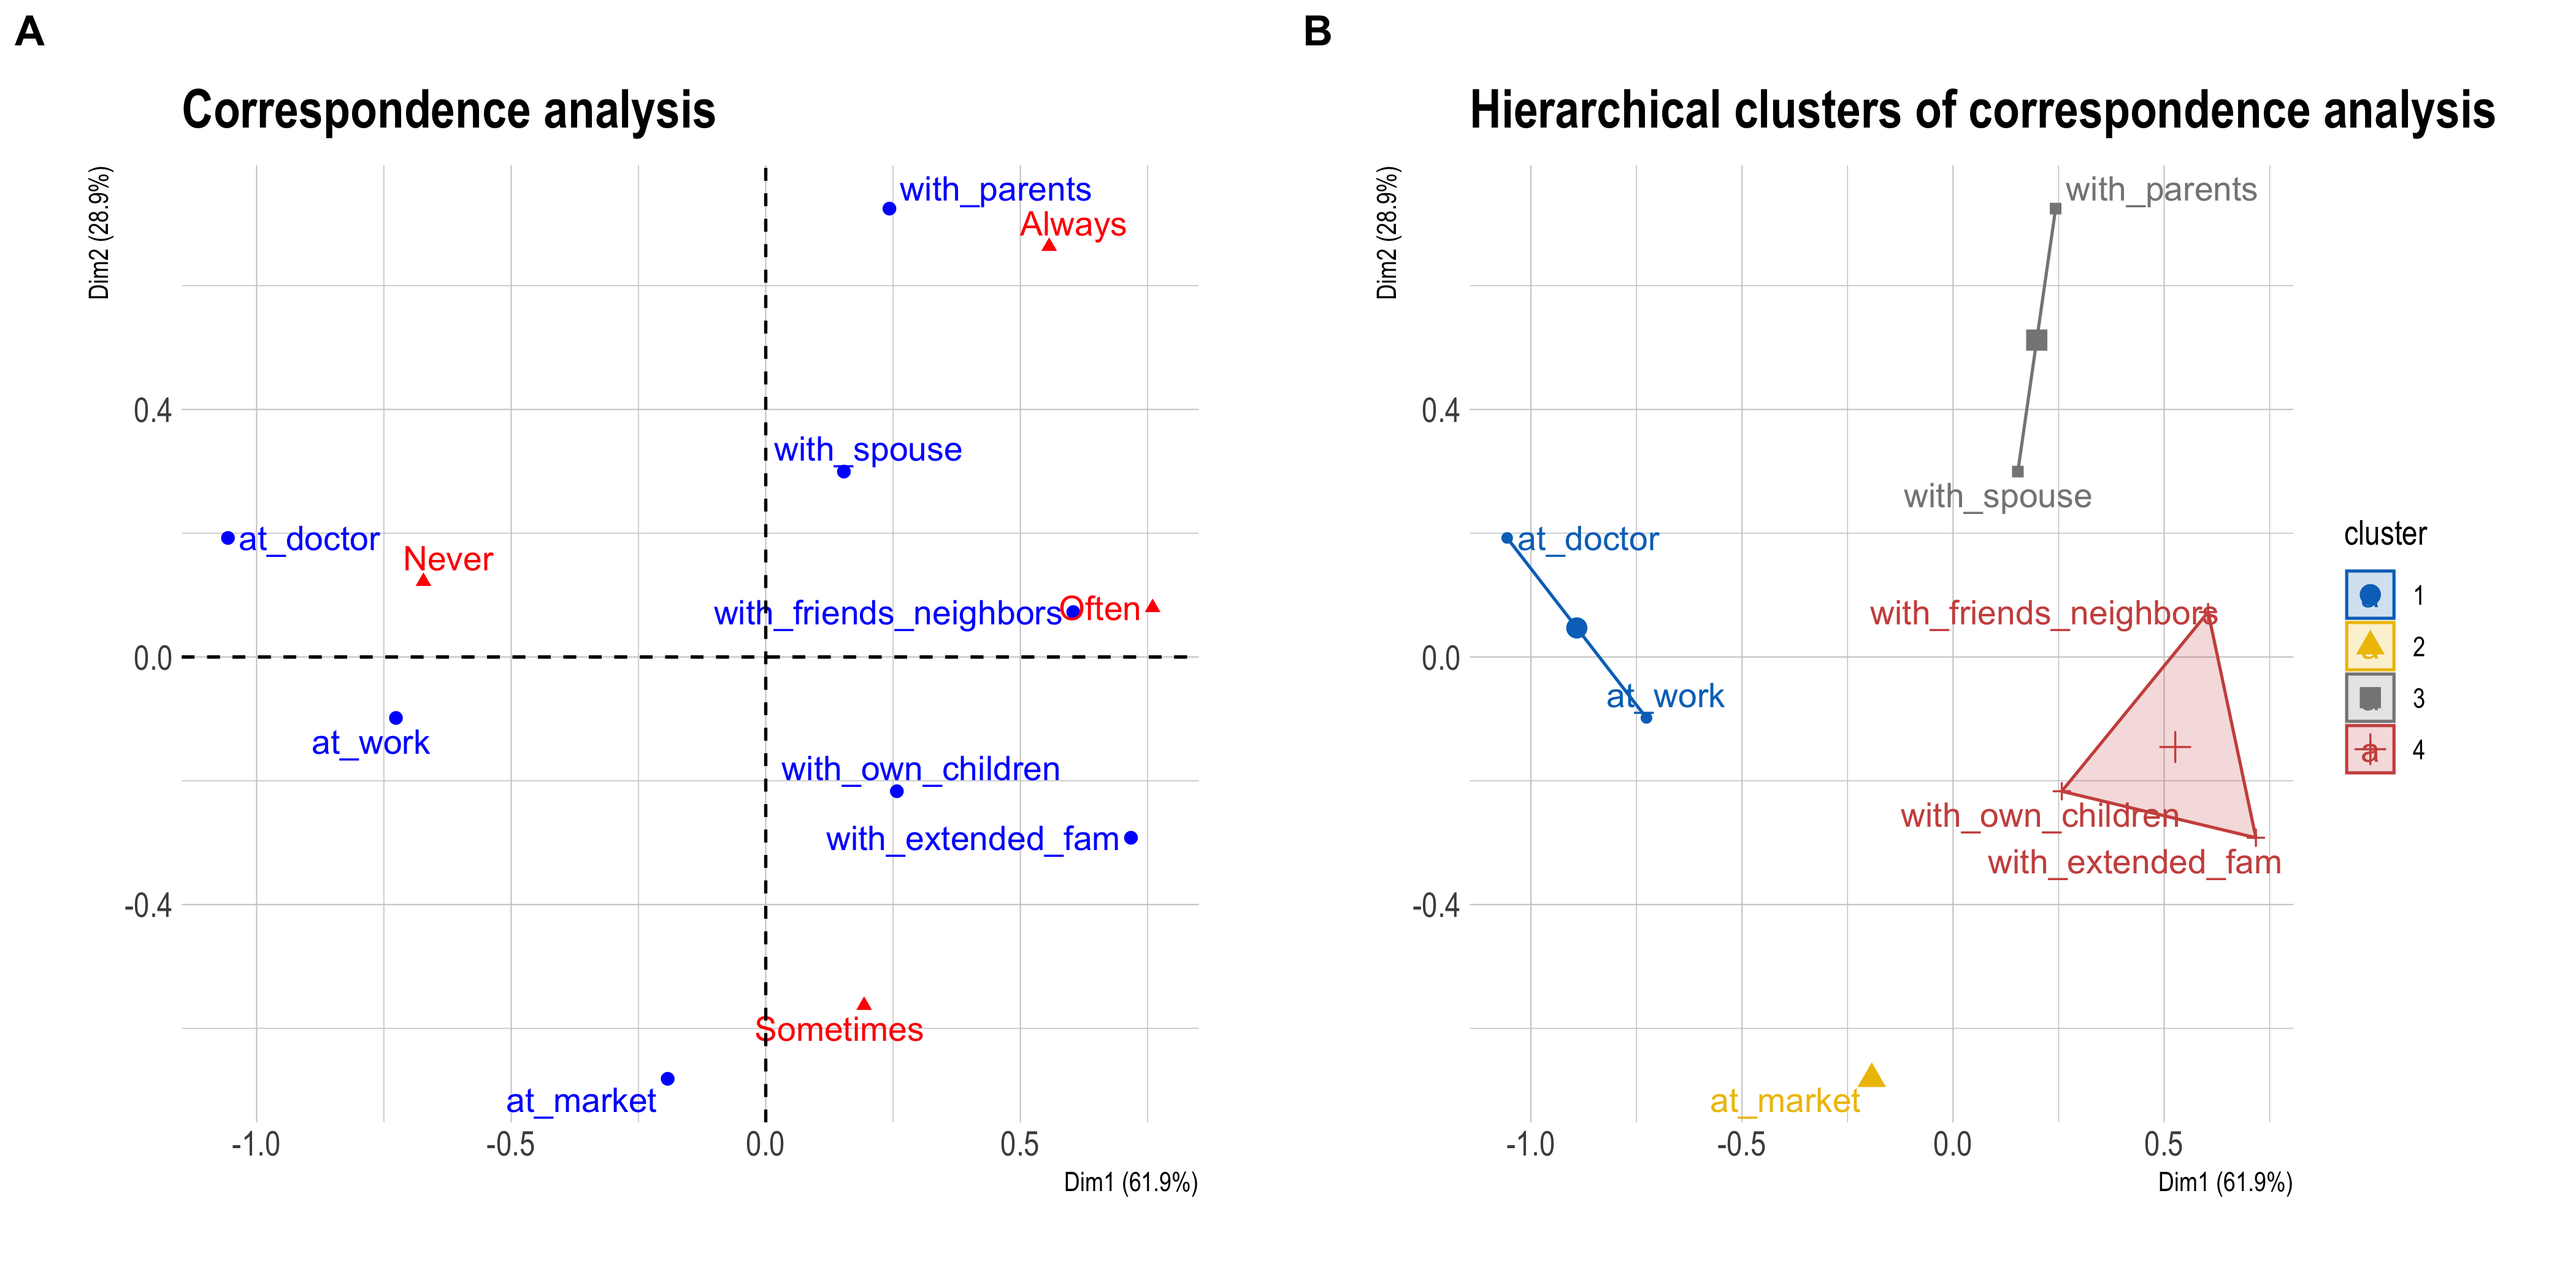
\includegraphics[width=0.7\textwidth]{ca-clusters-full.png} \vspace{-0.3in}\captionof{figure}{\footnotesize Correspondence analysis of domains of Tsova-Tush use (A) and hierarchical clusters of domains (B)}
\end{center}



}



%%%%%%



%\headerbox{Results (con't)}{name=locus3,column=2,row=0}{



%}



%%%%%



%----------------------------------------------------------------------------------------
%	CONCLUSION
%----------------------------------------------------------------------------------------

\headerbox{Conclusions}{name=conclusion,column=1,below=bhlm,span=2}{

\begin{singlespace}{\footnotesize
We found that widely cited estimates of Tsova-Tush speakers dramatically overrepresent the size of the present-day speakership. Even supposedly current sources still publish a speaker count that is likely 50 years old and 4--8 times too high, while failing to indicate the age or the provenance of the information. Recent publication dates, when associated with old estimates, give a false impression about the size of vulnerable and rapidly changing endangered language populations.\\ 



\vspace{-0.1in}Results from the language use survey presented a mixed picture of language use and attitudes. }\end{singlespace}
{\footnotesize
\begin{itemize}[leftmargin=*]\compresslist
\item \textbf{Overall use}: Older speakers were more likely than younger speakers to report using Tsova-Tush.
\item \textbf{Domains of use}: Older speakers reported using Tsova-Tush in a more diverse set of domains than younger speakers.
\begin{itemize}\compresslist
\item Domains of use fell along a scale (see e.g., \citealt{blommaertsociolinguistic2007}) where Tsova-Tush is used the least at translocal levels (doctor and work) and increasingly more often in more local levels. 
\item Even in the most local levels, with spouse or parents, Tsova-Tush was either \textit{always} or \textit{never} used.
\item Reported use was greater with extended family than with children.
\end{itemize}
\item \textbf{Importance of transmission}: Most respondents reported that it was ``somewhat important” or ``very important” for younger people to know Tsova-Tush.
\begin{itemize}\compresslist
\item Older respondents tended to rate transmission as more important than younger respondents.
\end{itemize}
\end{itemize}
}

{\footnotesize \begin{singlespace}Together, our updated speaker number estimates and results of the language use survey suggest that Tsova-Tush, while highly valued among speakers and still in use, is losing ground in all domains and is not being transmitted to children.\end{singlespace}}



}


%----------------------------------------------------------------------------------------
%	CONTACT INFORMATION
%----------------------------------------------------------------------------------------

\headerbox{Contact Information}{name=contact,column=2,below=conclusion}{ % This block is as tall as the references block
\scriptsize{
\begin{description}\compresslist
\item[Web] brynhauk.com, rentz.weebly.com
\item[Email] bhauk@hawaii.edu, rentzb@hawaii.edu
\item[Data \& Code] github.com/rentzb/icldc-bbl
\end{description}



}}

\headerbox{Acknowledgments}{name=ackno,column=1,below=conclusion,span=1}{
{\begin{singlespace}\scriptsize We thank the Bilinski Education Foundation for grant support and Dr.~Andrea Berez-Kroeker for comments. Thanks also to Revaz Orbetišvili and to Tsova-Tush respondents: {\georgianfont მადელ შუნ}. Errors are our own.}
\end{singlespace}
}


\end{poster}

\end{document}